\documentclass[a4paper, 14pt]{extarticle}

% Поля
%--------------------------------------
\usepackage{geometry}
\geometry{a4paper,tmargin=2cm,bmargin=2cm,lmargin=3cm,rmargin=1cm}
%--------------------------------------


%Russian-specific packages
%--------------------------------------
\usepackage[T2A]{fontenc}
\usepackage[utf8]{inputenc} 
\usepackage[english, main=russian]{babel}
%--------------------------------------

\usepackage{textcomp}

% Красная строка
%--------------------------------------
\usepackage{indentfirst}               
%--------------------------------------             

\newcommand{\T}{\mathcal{T}}

%Graphics
%--------------------------------------
\usepackage{graphicx}
\graphicspath{ {./images/} }
\usepackage{wrapfig}
%--------------------------------------

% Полуторный интервал
%--------------------------------------
\linespread{1.3}                    
%--------------------------------------

%Выравнивание и переносы
%--------------------------------------
% Избавляемся от переполнений
\sloppy
% Запрещаем разрыв страницы после первой строки абзаца
\clubpenalty=10000
% Запрещаем разрыв страницы после последней строки абзаца
\widowpenalty=10000
%--------------------------------------

%Списки
\usepackage{enumitem}

%Подписи
\usepackage{caption} 

%Гиперссылки
\usepackage{hyperref}

\hypersetup {
	unicode=true
}

%Рисунки
%--------------------------------------
\DeclareCaptionLabelSeparator*{emdash}{~--- }
\captionsetup[figure]{labelsep=emdash,font=onehalfspacing,position=bottom}
%--------------------------------------

\usepackage{tempora}


%Листинги
%--------------------------------------
\usepackage{listings}
\lstset{
  basicstyle=\ttfamily\footnotesize, 
  %basicstyle=\footnotesize\AnkaCoder,        % the size of the fonts that are used for the code
  breakatwhitespace=false,         % sets if automatic breaks shoulbd only happen at whitespace
  breaklines=true,                 % sets automatic line breaking
  captionpos=t,                    % sets the caption-position to bottom
  inputencoding=utf8,
  frame=single,                    % adds a frame around the code
  keepspaces=true,                 % keeps spaces in text, useful for keeping indentation of code (possibly needs columns=flexible)
  keywordstyle=\bf,       % keyword style
  numbers=left,                    % where to put the line-numbers; possible values are (none, left, right)
  numbersep=5pt,                   % how far the line-numbers are from the code
  xleftmargin=25pt,
  xrightmargin=25pt,
  showspaces=false,                % show spaces everywhere adding particular underscores; it overrides 'showstringspaces'
  showstringspaces=false,          % underline spaces within strings only
  showtabs=false,                  % show tabs within strings adding particular underscores
  stepnumber=1,                    % the step between two line-numbers. If it's 1, each line will be numbered
  tabsize=2,                       % sets default tabsize to 8 spaces
  title=\lstname                   % show the filename of files included with \lstinputlisting; also try caption instead of title
}

%--------------------------------------

%%% Математические пакеты %%%
%--------------------------------------
\usepackage{amsthm,amsfonts,amsmath,amssymb,amscd}  % Математические дополнения от AMS
\usepackage{mathtools}                              % Добавляет окружение multlined
\usepackage[perpage]{footmisc}
%--------------------------------------

%--------------------------------------
%			НАЧАЛО ДОКУМЕНТА
%--------------------------------------

\begin{document}

%--------------------------------------
%			ТИТУЛЬНЫЙ ЛИСТ
%--------------------------------------
\begin{titlepage}
\thispagestyle{empty}
\newpage


%Шапка титульного листа
%--------------------------------------
\vspace*{-60pt}
\hspace{-65pt}
\begin{minipage}{0.3\textwidth}
\hspace*{-20pt}\centering

\includegraphics[width=\textwidth]{emblem}
\end{minipage}
\begin{minipage}{0.67\textwidth}\small \textbf{
\vspace*{-0.7ex}
\hspace*{-6pt}\centerline{Министерство науки и высшего образования Российской Федерации}
\vspace*{-0.7ex}
\centerline{Федеральное государственное бюджетное образовательное учреждение }
\vspace*{-0.7ex}
\centerline{высшего образования}
\vspace*{-0.7ex}
\centerline{<<Московский государственный технический университет}
\vspace*{-0.7ex}
\centerline{имени Н.Э. Баумана}
\vspace*{-0.7ex}
\centerline{(национальный исследовательский университет)>>}
\vspace*{-0.7ex}
\centerline{(МГТУ им. Н.Э. Баумана)}}
\end{minipage}
%--------------------------------------

%Полосы
%--------------------------------------
\vspace{-25pt}
\hspace{-35pt}\rule{\textwidth}{2.3pt}

\vspace*{-20.3pt}
\hspace{-35pt}\rule{\textwidth}{0.4pt}
%--------------------------------------

\vspace{1.5ex}
\hspace{-35pt} \noindent \small ФАКУЛЬТЕТ\hspace{80pt} <<Информатика и системы управления>>

\vspace*{-16pt}
\hspace{47pt}\rule{0.83\textwidth}{0.4pt}

\vspace{0.5ex}
\hspace{-35pt} \noindent \small КАФЕДРА\hspace{50pt} <<Теоретическая информатика и компьютерные технологии>>

\vspace*{-16pt}
\hspace{30pt}\rule{0.866\textwidth}{0.4pt}
  
\vspace{11em}

\begin{center}
\Large {\bf Лабораторная работа № 2} \\ 
\large {\bf по курсу <<Теория формальных языков>>} \\
% \large «Моделирование данных с использованием модели семантических объектов» 
\end{center}\normalsize

\vspace{8em}


\begin{flushright}
  {Студент группы ИУ9-51Б Санталов Д.А. \hspace*{15pt}\\ 
  \vspace{2ex}
  Преподаватель Непейвода А. Н.\hspace*{15pt}}
\end{flushright}

\bigskip

\vfill
 

\begin{center}
\textsl{Москва 2025}
\end{center}
\end{titlepage}
%--------------------------------------
%		КОНЕЦ ТИТУЛЬНОГО ЛИСТА
%--------------------------------------

\renewcommand{\ttdefault}{pcr}

\setlength{\tabcolsep}{3pt}
\newpage
\setcounter{page}{2}

% Оглавление
\tableofcontents
\newpage

\section{Постановка задачи}\label{Sect::task}
По имеющемуся академическому регулярному выражению построить:
\begin{enumerate}
    \item минимальный ДКА, распознающий его язык (минимальность обосновать
таблицей классов эквивалентности)
    \item возможно малый НКА, распознающий его язык. Возможно малый переключающийся (с конъюнкцией) КА, распознающий его язык. Частично обосновать таблицами множеств классов эквивалентности
    \item расширенное регулярное выражение, распознающее тот же язык. В расширенном выражении можно использовать:
    \begin{itemize}
        \item wildcard-операцию . для замены произвольного символа алфавита;
        \item положительную итерацию $\tau^+$ и опцию $\tau?.\tau^+=\tau\tau^*, \tau? = (\tau | \varepsilon)$;
        \item операции предпросмотра $\tau_0 (?=\tau_1)\tau_2 \equiv \tau_0((\tau_1.^*\cap \tau_2)$ и ретроспективной проверки $\tau_0 (? <= \tau_1)\tau_2 \equiv (\tau_0 \cap (\tau_1.^*))\tau_2$, а также их отрицательные версии $\tau_0(?! \tau_1)\tau_2 \equiv \tau_0(\overline{(\tau_1.^*)} \cap \tau_2)$ и $\tau_0(?<! \tau_1)\tau_2 \equiv (\tau_0 \cap \overline{(\tau_1.^*)})\tau_2$;
        \item классы букв $[c_1 \ldots c_k] \equiv (c_1 |c_2 | \ldots |c_k )$ и их дополнения $[ˆc_1 \ldots c_k]$.
        \item (обязательно) маркеры начала и конца выражения \textasciicircum \; и \$.
    \end{itemize}

    Академическое регулярное выражение: 
    
    $(abc|bac|cba|bca|acb)^*aa(a|b|c)(a|b)(b|c)(a|c)$.
\end{enumerate}
\section{Основная часть}\label{Sect::realisation}

\subsection{НКА}
На основе академического регулярного выражения был построен НКА в первом приближении (NFA\_dtaft.svg):
\begin{center}
    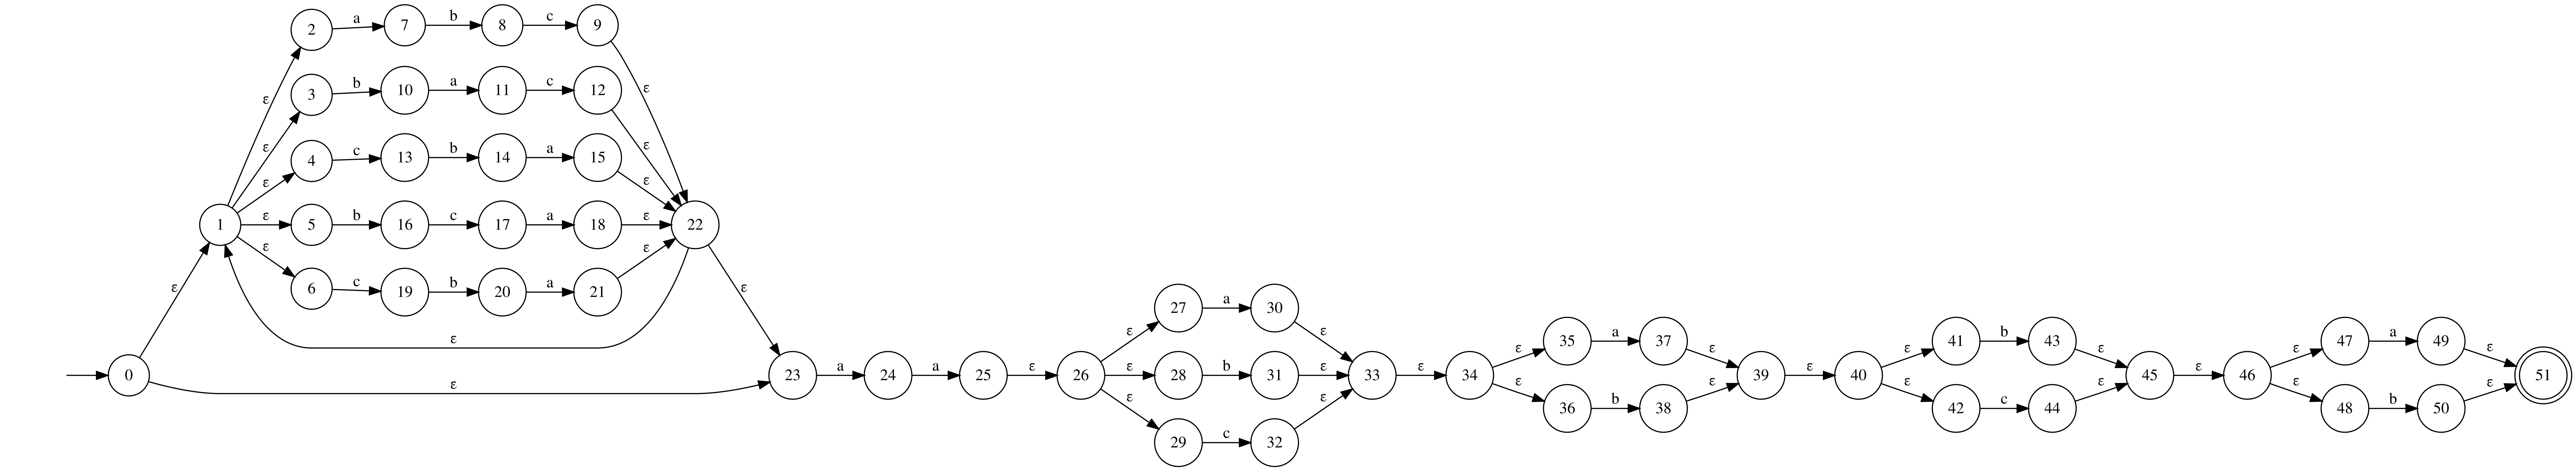
\includegraphics[width=\linewidth]{images/NFA_draft.png}
\end{center}

Затем был построен возможно минимальный НКА (minNFA.svg):
\begin{center}
    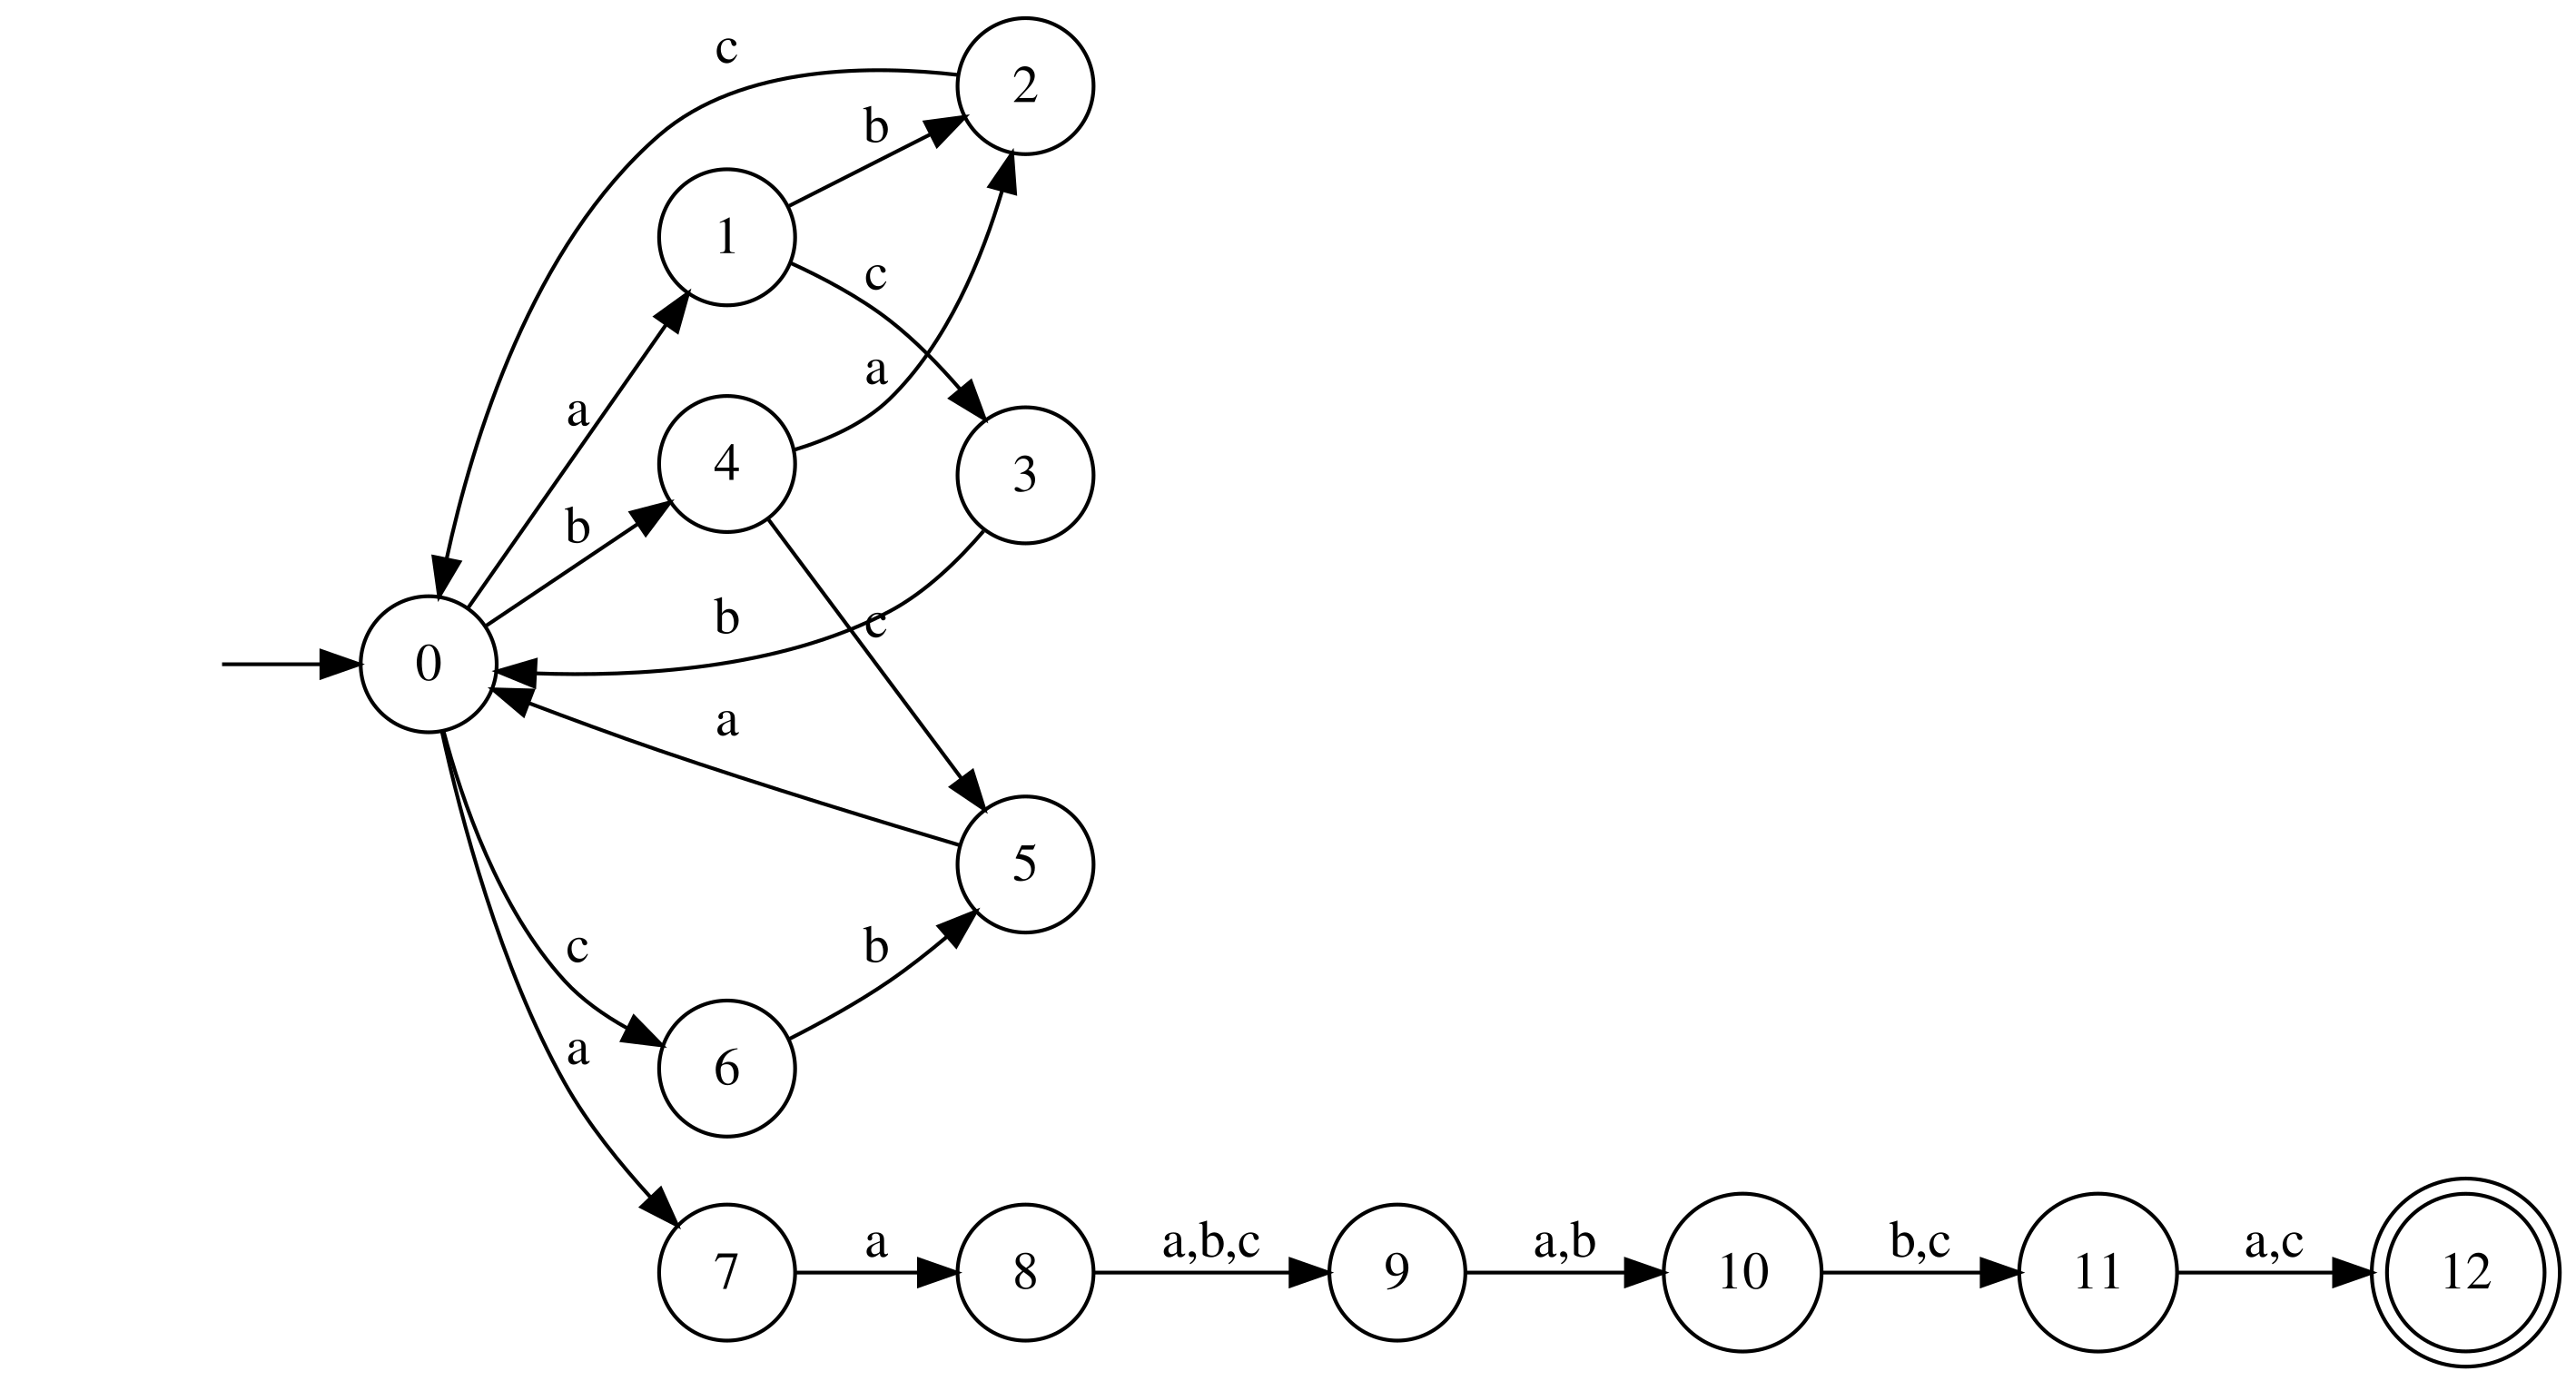
\includegraphics[width=\linewidth]{images/minNFA.png}
\end{center}

\textbf{Обоснование минимальности НКА}\\

\hspace*{-2cm}
\begin{tabular}{|c|c|c|c|c|c|c|c|c|c|c|c|c|}
\hline 
 & aaaaba & bcaaabcc & acaacbca & baaabbba & aaba & baababa & caababa & aaaaaba & aba & ba & a & $\varepsilon$ \\
\hline
$\varepsilon$ & 1 &0 & 0 & 0 & 0 & 0 & 0 & 0 & 0 & 0 & 0 & 0 \\
\hline
a & 0 & 1 & 0 & 0 & 0 & 0 & 0 & 0 & 0 & 0 & 0 & 0 \\
\hline
b & 0 & 0 & 1 & 0 & 0 & 0 & 0 & 0 & 0 & 0 & 0 & 0 \\
\hline
c & 0 & 0 & 0 & 1 & 0 & 0 & 0 & 0 & 0 & 0 & 0 & 0 \\
\hline
aa & 0 &  0 & 0 & 0 & 1 & 0 & 0 & 0 & 0 & 0 & 0 & 0 \\
\hline
ac & 0 & 0 & 0 & 0 & 0 & 1 & 0 & 0 & 0 & 0 & 0 & 0 \\
\hline
ab & 0& 0 & 0 & 0 & 0 & 0 & 1 & 0 & 0 & 0 & 0 & 0 \\
\hline
bc & 0 & 0 & 0 & 0 & 0 & 0 & 0 & 1 & 0 & 0 & 0 & 0 \\
\hline
aaa & 0 & 0 & 0 & 0 & 0 & 0 & 0 & 0 & 1 & 0 & 0 & 0 \\
\hline
aaaa & 0 & 0 & 0 & 0 & 0 & 0 & 0 & 0 & 0 & 1 & 0 & 0 \\
\hline
aaaab & 0 & 0 & 0 & 0 & 0 & 0 & 0 & 0 & 0 & 0 & 1 & 0 \\
\hline
aaaaba & 0 & 0 & 0 & 0 & 0 & 0 & 0 & 0 & 0 & 0 & 0 & 1 \\
\hline
\end{tabular}

\subsection{ДКА}
На основе академического регулярного выражения и его представления в виде НКА был построен и минимизирован ДКА (minDFA.svg):

\begin{center}
    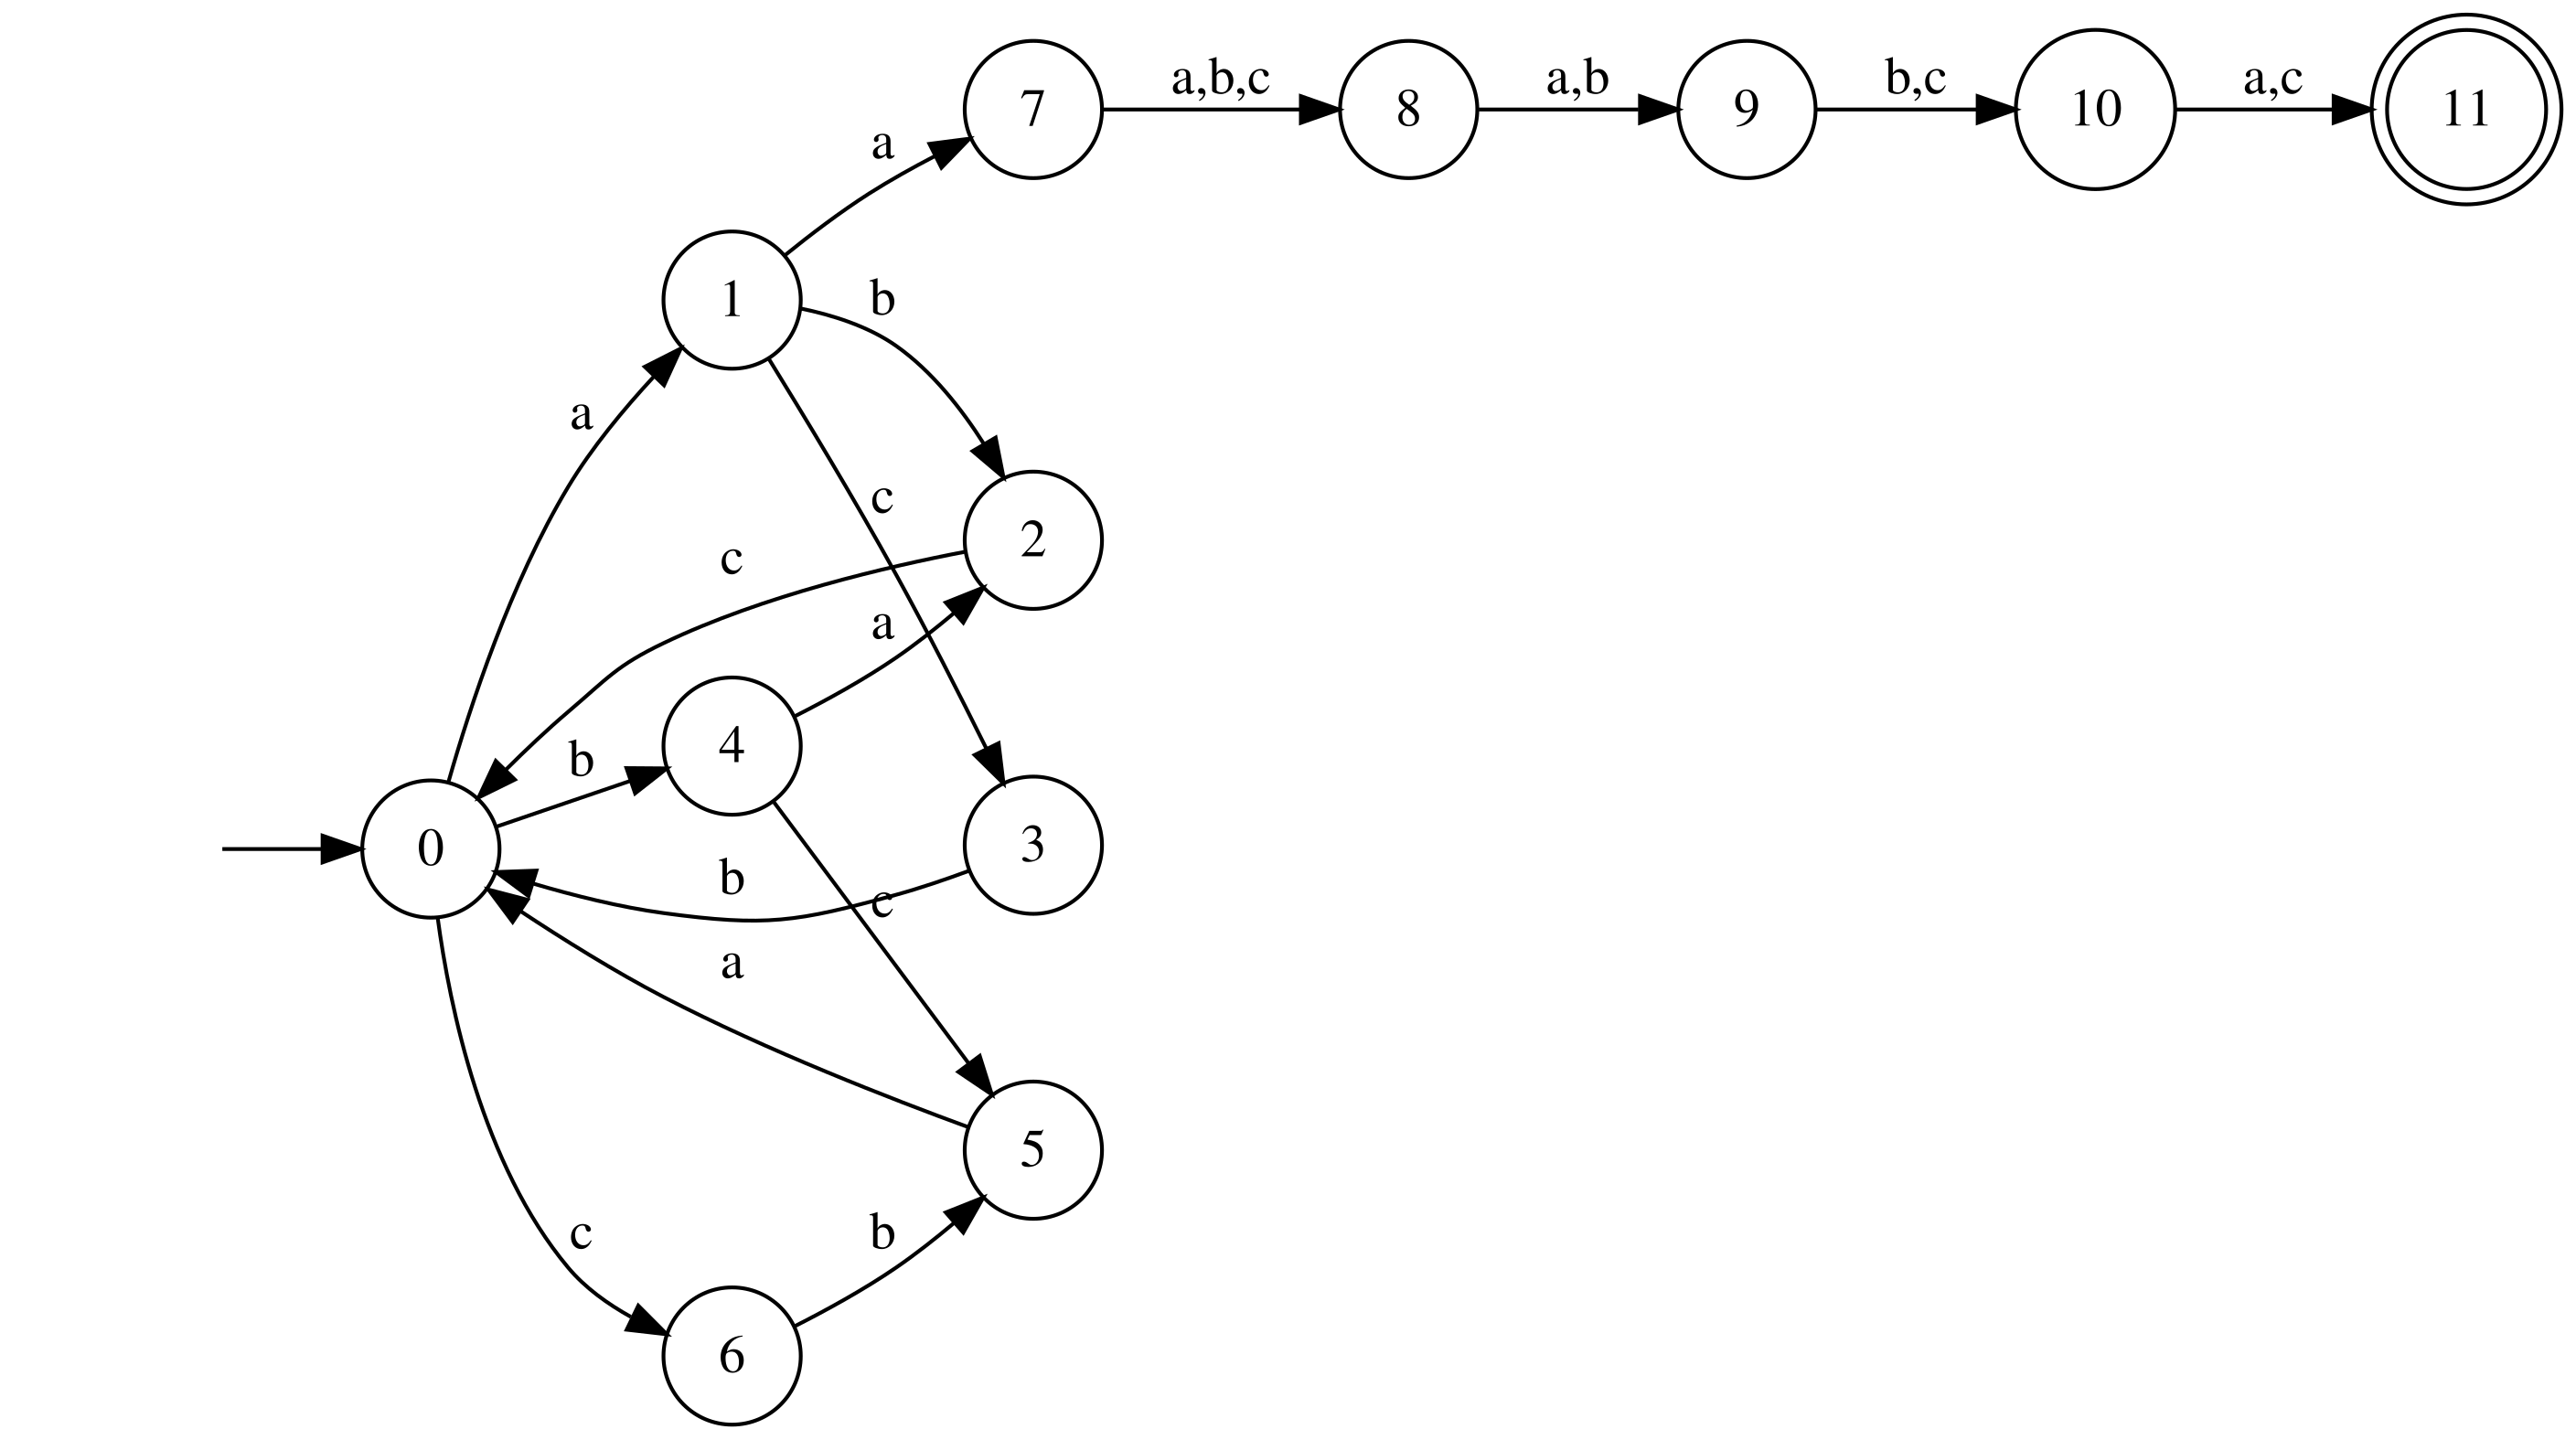
\includegraphics[width=\linewidth]{images/minDFA.png}
\end{center}

% \clearpage
\textbf{Обоснование минимальности ДКА}\\

\hspace*{-2cm}
\begin{tabular}{|c|c|c|c|c|c|c|c|c|c|c|c|c|}
\hline 
 & aaaaba & bcaaabcc & acaacbca & baaabbba & aaba & baababa & caababa & aaaaaba & aba & ba & a & $\varepsilon$ \\
\hline
$\varepsilon$ & 1 &0 & 0 & 0 & 0 & 0 & 0 & 0 & 0 & 0 & 0 & 0 \\
\hline
a & 0 & 1 & 0 & 0 & 0 & 0 & 0 & 0 & 0 & 0 & 0 & 0 \\
\hline
b & 0 & 0 & 1 & 0 & 0 & 0 & 0 & 0 & 0 & 0 & 0 & 0 \\
\hline
c & 0 & 0 & 0 & 1 & 0 & 0 & 0 & 0 & 0 & 0 & 0 & 0 \\
\hline
aa & 0 &  0 & 0 & 0 & 1 & 0 & 0 & 0 & 0 & 0 & 0 & 0 \\
\hline
ac & 0 & 0 & 0 & 0 & 0 & 1 & 0 & 0 & 0 & 0 & 0 & 0 \\
\hline
ab & 0& 0 & 0 & 0 & 0 & 0 & 1 & 0 & 0 & 0 & 0 & 0 \\
\hline
bc & 0 & 0 & 0 & 0 & 0 & 0 & 0 & 1 & 0 & 0 & 0 & 0 \\
\hline
aaa & 0 & 0 & 0 & 0 & 0 & 0 & 0 & 0 & 1 & 0 & 0 & 0 \\
\hline
aaaa & 0 & 0 & 0 & 0 & 0 & 0 & 0 & 0 & 0 & 1 & 0 & 0 \\
\hline
aaaab & 0 & 0 & 0 & 0 & 0 & 0 & 0 & 0 & 0 & 0 & 1 & 0 \\
\hline
aaaaba & 0 & 0 & 0 & 0 & 0 & 0 & 0 & 0 & 0 & 0 & 0 & 1 \\
\hline
\end{tabular}

\subsection{ПКА}
На основе академического регулярного выражения был построен переключающийся (с конъюнкцией) конечный автомат (AFA.svg), распознающий язык исходного регулярного выражения:

\begin{center}
    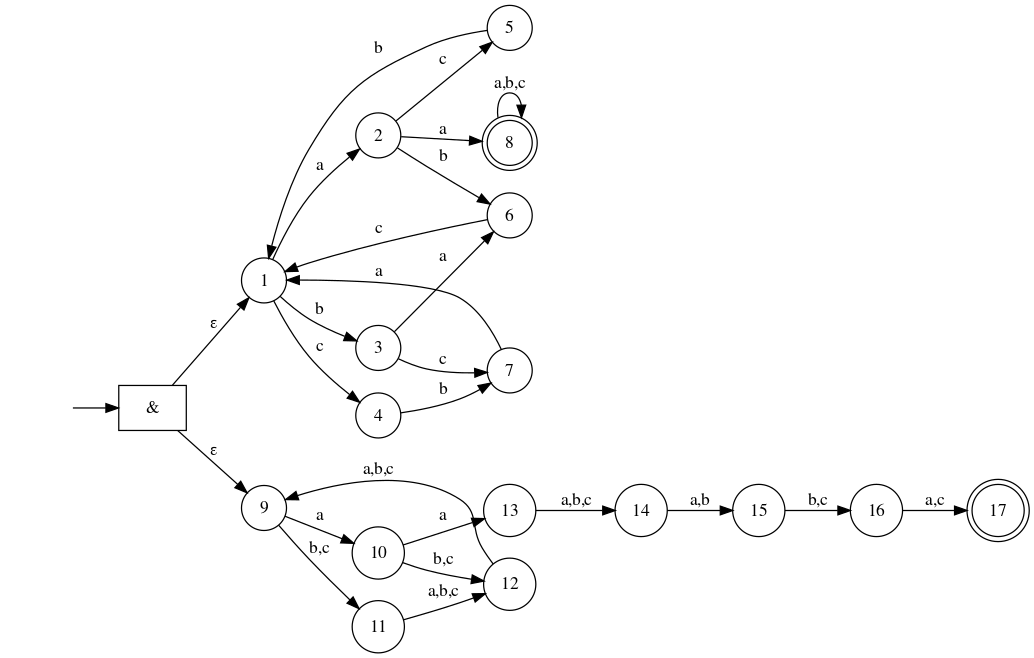
\includegraphics[width=\linewidth]{images/AFA.png}
\end{center}

\textbf{Обоснование минимальности ПКА}\\

\begin{tabular}{|c|c|c|c|c|c|c|c|c|c|c|c|c|}
\hline 
 & $\varepsilon$ & a  \\
\hline
aaaab & 0 & 1 \\
\hline
$\varepsilon$ & 0 & 0 \\
\hline
\end{tabular}

\subsection{Расширенное регулярное выражение}

$\textasciicircum ((a(bc|cb)|b(ac|ca)|cba)^+)?aa.(?! c).(?! a).(?! b).\$$

Итерация Клини $(abc|bac|cba|bca|acb)^*$ -- это повторение несколько раз  блока $(abc|bac|cba|bca|acb)$ или $\varepsilon$. Поэтому можем представить повторение нескольких раз блока $(abc|bac|cba|bca|acb)$ в виде $(abc|bac|cba|bca|acb)^+$, а возможность получения $\varepsilon$ из итерации Клини -- так: $((abc|bac|cba|bca|acb)^+)?$.

Поскольку символы алфавита -- $a, b, c$, то блок $(a|b|c)$ может быть заменен символом ``$.$``.


Блоки $(a|b)$, $(b|c)$ и $(a|c)$ заменяем по определению на $\left[ab\right],\left[bc\right]$ и $\left[ac\right]$.

\end{document}

